% Created 2021-06-30 on 14:38
% Intended LaTeX compiler: pdflatex
\documentclass[12pt]{article}

%%%% settings when exporting code %%%% 

\usepackage{listings}
\lstdefinestyle{code-small}{
backgroundcolor=\color{white}, % background color for the code block
basicstyle=\ttfamily\small, % font used to display the code
commentstyle=\color[rgb]{0.5,0,0.5}, % color used to display comments in the code
keywordstyle=\color{black}, % color used to highlight certain words in the code
numberstyle=\ttfamily\tiny\color{gray}, % color used to display the line numbers
rulecolor=\color{black}, % color of the frame
stringstyle=\color[rgb]{0,.5,0},  % color used to display strings in the code
breakatwhitespace=false, % sets if automatic breaks should only happen at whitespace
breaklines=true, % sets automatic line breaking
columns=fullflexible,
frame=single, % adds a frame around the code (non,leftline,topline,bottomline,lines,single,shadowbox)
keepspaces=true, % % keeps spaces in text, useful for keeping indentation of code
literate={~}{$\sim$}{1}, % symbol properly display via latex
numbers=none, % where to put the line-numbers; possible values are (none, left, right)
numbersep=10pt, % how far the line-numbers are from the code
showspaces=false,
showstringspaces=false,
stepnumber=1, % the step between two line-numbers. If it's 1, each line will be numbered
tabsize=1,
xleftmargin=0cm,
emph={anova,apply,class,coef,colnames,colNames,colSums,dim,dcast,for,ggplot,head,if,ifelse,is.na,lapply,list.files,library,logLik,melt,plot,require,rowSums,sapply,setcolorder,setkey,str,summary,tapply},
aboveskip = \medskipamount, % define the space above displayed listings.
belowskip = \medskipamount, % define the space above displayed listings.
lineskip = 0pt} % specifies additional space between lines in listings
\lstset{style=code-small}
%%%% packages %%%%%

\usepackage[utf8]{inputenc}
\usepackage[T1]{fontenc}
\usepackage{lmodern}
\usepackage{textcomp}
\usepackage{color}
\usepackage{graphicx}
\usepackage{grffile}
\usepackage{wrapfig}
\usepackage{rotating}
\usepackage{longtable}
\usepackage{multirow}
\usepackage{multicol}
\usepackage{changes}
\usepackage{pdflscape}
\usepackage{geometry}
\usepackage[normalem]{ulem}
\usepackage{amssymb}
\usepackage{amsmath}
\usepackage{amsfonts}
\usepackage{dsfont}
\usepackage{array}
\usepackage{ifthen}
\usepackage{hyperref}
\usepackage{natbib}
\RequirePackage{setspace} % to modify the space between lines - incompatible with footnote in beamer
\renewcommand{\baselinestretch}{1.1}
\geometry{top=1cm}
\usepackage{titlesec}
\usepackage{etoolbox}

\makeatletter
\patchcmd{\ttlh@hang}{\parindent\z@}{\parindent\z@\leavevmode}{}{}
\patchcmd{\ttlh@hang}{\noindent}{}{}{}
\makeatother
\RequirePackage{colortbl} % arrayrulecolor to mix colors
\definecolor{myorange}{rgb}{1,0.2,0}
\definecolor{mypurple}{rgb}{0.7,0,8}
\definecolor{mycyan}{rgb}{0,0.6,0.6}
\newcommand{\lightblue}{blue!50!white}
\newcommand{\darkblue}{blue!80!black}
\newcommand{\darkgreen}{green!50!black}
\newcommand{\darkred}{red!50!black}
\definecolor{gray}{gray}{0.5}
\hypersetup{
citecolor=[rgb]{0,0.5,0},
urlcolor=[rgb]{0,0,0.5},
linkcolor=[rgb]{0,0,0.5},
}
\newenvironment{note}{\small \color{gray}\fontfamily{lmtt}\selectfont}{\par}
\newenvironment{activity}{\color{orange}\fontfamily{qzc}\selectfont}{\par}
\RequirePackage{pifont}
\RequirePackage{relsize}
\newcommand{\Cross}{{\raisebox{-0.5ex}%
{\relsize{1.5}\ding{56}}}\hspace{1pt} }
\newcommand{\Valid}{{\raisebox{-0.5ex}%
{\relsize{1.5}\ding{52}}}\hspace{1pt} }
\newcommand{\CrossR}{ \textcolor{red}{\Cross} }
\newcommand{\ValidV}{ \textcolor{green}{\Valid} }
\usepackage{stackengine}
\usepackage{scalerel}
\newcommand\Warning[1][3ex]{%
\renewcommand\stacktype{L}%
\scaleto{\stackon[1.3pt]{\color{red}$\triangle$}{\tiny\bfseries !}}{#1}%
\xspace
}
\newcommand\Rlogo{\textbf{\textsf{R}}\xspace} %
\RequirePackage{fancyvrb}
\DefineVerbatimEnvironment{verbatim}{Verbatim}{fontsize=\small,formatcom = {\color[rgb]{0.5,0,0}}}
\RequirePackage{enumitem} % better than enumerate
\RequirePackage{epstopdf} % to be able to convert .eps to .pdf image files
\RequirePackage{capt-of} %
\RequirePackage{caption} % newlines in graphics
\RequirePackage{tikz-cd} % graph
\RequirePackage{booktabs} % for nice lines in table (e.g. toprule, bottomrule, midrule, cmidrule)
\RequirePackage{amsmath}
\RequirePackage{algorithm}
\RequirePackage[noend]{algpseudocode}
\RequirePackage{dsfont}
\RequirePackage{amsmath,stmaryrd,graphicx}
\RequirePackage{prodint} % product integral symbol (\PRODI)
\usepackage{ifthen}
\usepackage{xifthen}
\usepackage{xargs}
\usepackage{xspace}
\newcommand\defOperator[7]{%
\ifthenelse{\isempty{#2}}{
\ifthenelse{\isempty{#1}}{#7{#3}#4}{#7{#3}#4 \left#5 #1 \right#6}
}{
\ifthenelse{\isempty{#1}}{#7{#3}#4_{#2}}{#7{#3}#4_{#1}\left#5 #2 \right#6}
}
}
\newcommand\defUOperator[5]{%
\ifthenelse{\isempty{#1}}{
#5\left#3 #2 \right#4
}{
\ifthenelse{\isempty{#2}}{\underset{#1}{\operatornamewithlimits{#5}}}{
\underset{#1}{\operatornamewithlimits{#5}}\left#3 #2 \right#4}
}
}
\newcommand{\defBoldVar}[2]{
\ifthenelse{\equal{#2}{T}}{\boldsymbol{#1}}{\mathbf{#1}}
}
\newcommandx\Esp[2][1=,2=]{\defOperator{#1}{#2}{E}{}{\lbrack}{\rbrack}{\mathbb}}
\newcommandx\Prob[2][1=,2=]{\defOperator{#1}{#2}{P}{}{\lbrack}{\rbrack}{\mathbb}}
\newcommandx\Qrob[2][1=,2=]{\defOperator{#1}{#2}{Q}{}{\lbrack}{\rbrack}{\mathbb}}
\newcommandx\Var[2][1=,2=]{\defOperator{#1}{#2}{V}{ar}{\lbrack}{\rbrack}{\mathbb}}
\newcommandx\Cov[2][1=,2=]{\defOperator{#1}{#2}{C}{ov}{\lbrack}{\rbrack}{\mathbb}}
\newcommandx\Binom[2][1=,2=]{\defOperator{#1}{#2}{B}{}{(}{)}{\mathcal}}
\newcommandx\Gaus[2][1=,2=]{\defOperator{#1}{#2}{N}{}{(}{)}{\mathcal}}
\newcommandx\Wishart[2][1=,2=]{\defOperator{#1}{#2}{W}{ishart}{(}{)}{\mathcal}}
\newcommandx\Likelihood[2][1=,2=]{\defOperator{#1}{#2}{L}{}{(}{)}{\mathcal}}
\newcommandx\logLikelihood[2][1=,2=]{\defOperator{#1}{#2}{\ell}{}{(}{)}{}}
\newcommandx\Information[2][1=,2=]{\defOperator{#1}{#2}{I}{}{(}{)}{\mathcal}}
\newcommandx\Score[2][1=,2=]{\defOperator{#1}{#2}{S}{}{(}{)}{\mathcal}}
\newcommandx\Vois[2][1=,2=]{\defOperator{#1}{#2}{V}{}{(}{)}{\mathcal}}
\newcommandx\IF[2][1=,2=]{\defOperator{#1}{#2}{IF}{}{(}{)}{\mathcal}}
\newcommandx\Ind[1][1=]{\defOperator{}{#1}{1}{}{(}{)}{\mathds}}
\newcommandx\Max[2][1=,2=]{\defUOperator{#1}{#2}{(}{)}{min}}
\newcommandx\Min[2][1=,2=]{\defUOperator{#1}{#2}{(}{)}{max}}
\newcommandx\argMax[2][1=,2=]{\defUOperator{#1}{#2}{(}{)}{argmax}}
\newcommandx\argMin[2][1=,2=]{\defUOperator{#1}{#2}{(}{)}{argmin}}
\newcommandx\cvD[2][1=D,2=n \rightarrow \infty]{\xrightarrow[#2]{#1}}
\newcommandx\Hypothesis[2][1=,2=]{
\ifthenelse{\isempty{#1}}{
\mathcal{H}
}{
\ifthenelse{\isempty{#2}}{
\mathcal{H}_{#1}
}{
\mathcal{H}^{(#2)}_{#1}
}
}
}
\newcommandx\dpartial[4][1=,2=,3=,4=\partial]{
\ifthenelse{\isempty{#3}}{
\frac{#4 #1}{#4 #2}
}{
\left.\frac{#4 #1}{#4 #2}\right\rvert_{#3}
}
}
\newcommandx\dTpartial[3][1=,2=,3=]{\dpartial[#1][#2][#3][d]}
\newcommandx\ddpartial[3][1=,2=,3=]{
\ifthenelse{\isempty{#3}}{
\frac{\partial^{2} #1}{\partial #2^2}
}{
\frac{\partial^2 #1}{\partial #2\partial #3}
}
}
\newcommand\Real{\mathbb{R}}
\newcommand\Rational{\mathbb{Q}}
\newcommand\Natural{\mathbb{N}}
\newcommand\trans[1]{{#1}^\intercal}%\newcommand\trans[1]{{\vphantom{#1}}^\top{#1}}
\newcommand{\independent}{\mathrel{\text{\scalebox{1.5}{$\perp\mkern-10mu\perp$}}}}
\newcommand\half{\frac{1}{2}}
\newcommand\normMax[1]{\left|\left|#1\right|\right|_{max}}
\newcommand\normTwo[1]{\left|\left|#1\right|\right|_{2}}
\newcommand\Veta{\boldsymbol{\eta}}
\newcommand\VX{\mathbf{X}}
\newcommand\sample{\chi}
\newcommand\Hspace{\mathcal{H}}
\newcommand\Tspace{\mathcal{T}}
\author{Brice Ozenne}
\date{\today}
\title{Efficient baseline adjustment in a randomized trial}
\hypersetup{
 colorlinks=true,
 pdfauthor={Brice Ozenne},
 pdftitle={Efficient baseline adjustment in a randomized trial},
 pdfkeywords={},
 pdfsubject={},
 pdfcreator={Emacs 27.1 (Org mode 9.4.5)},
 pdflang={English}
 }
\begin{document}

\maketitle
Disclaimer: this note is a compilation of section 5.4 of
\cite{tsiatis2007semiparametric}, \cite{zhang2010increasing} and a note by
Torben Martinussen.

\section{Motivation, objective, and notations}
\label{sec:orgcdf2321}

We consider a randomized trial with a single binary or continuous
outcome (\(Y\)), two treatment arms: placebo (\(A=0\)) and active
(\(A=1\)), and some baseline variables (\(Z\)). There are in total
\(n=n_0+n_1\) patients, \(n_0\) in the placebo arm and \(n_1\) in the
treatment arm. The observed data is therefore \(\sample =
\left(\sample_i\right)_{i \in \{1,\ldots,n\}} =
\left(Y_i,A_i,Z_i\right)_{i \in \{1,\ldots,n\}}\).

\bigskip 

Our parameter of interest is the average difference in outcome:
\begin{align*}
\psi = \Esp[Y|A=1] - \Esp[Y|A=0] = \mu_1 - \mu_0
\end{align*}
which we would like to estimate as efficiently as possible by making
use of the baseline variables. We denote \(\pi=\Prob[A=1]\) which is
known.

\section{Naive estimator}
\label{sec:orgd815e35}

A possible estimator for \(\psi\) is:
\begin{align*}
\hat{\psi}_n = \frac{\sum_{i=1}^n A_i Y_i}{\sum_{i=1}^n A_i} - \frac{\sum_{i=1}^n (1-A_i) Y_i}{\sum_{i=1}^n (1-A_i)}
\end{align*}
which satisfies the following decomposition:
\begin{align*}
\sqrt{n}\left(\hat{\psi}_n - \psi\right) 
&= \sqrt{n} \left(\frac{\sum_{i=1}^n A_i Y_i}{\sum_{i=1}^n A_i} - \mu_1\right) - \sqrt{n} \left(\frac{\sum_{i=1}^n (1-A_i) Y_i}{\sum_{i=1}^n (1-A_i)} - \mu_0\right) \\
&= \sqrt{n} \frac{\sum_{i=1}^n A_i (Y_i-\mu_1)}{\sum_{i=1}^n A_i}  - \sqrt{n} \frac{\sum_{i=1}^n (1-A_i) (Y_i-\mu_0)}{\sum_{i=1}^n (1-A_i)} \\
&= \frac{1}{\sqrt{n}} \frac{\sum_{i=1}^n A_i (Y_i-\mu_1)}{\frac{1}{n}\sum_{i=1}^n A_i}  - \frac{1}{\sqrt{n}} \frac{\sum_{i=1}^n (1-A_i) (Y_i-\mu_0)}{\frac{1}{n}\sum_{i=1}^n (1-A_i)} \\
&= \frac{1}{\sqrt{n}} \sum_{i=1}^n \frac{A_i}{\pi} \left(Y_i - \mu_1\right) - \frac{(1-A_i)}{1-\pi}\left(Y_i - \mu_0\right) + o_p(1) \\
&= \frac{1}{\sqrt{n}} \sum_{i=1}^n \IF_{\hat{\mu}_1}(\sample_i) - \IF_{\hat{\mu}_0}(\sample_i)+ o_p(1) \\
&= \frac{1}{\sqrt{n}} \sum_{i=1}^n \IF_{\hat{\psi}}(\sample_i) + o_p(1)
\end{align*}
where \(\IF_x\) denotes the influence function associated with the
estimator \(x\).

\section{Derivation of the semi-parametric efficient estimator}
\label{sec:org91b19ae}

\subsection{Geometry of the set of all influence function}
\label{sec:orgbd9b5f5}
The log-likelihood can be decomposed as:
\begin{align*}
\log(f(Y,A,Z)) = \log(f(Y|A,Z)) + \log(f(A|Z)) + \log(f(Z))
\end{align*}
While \(f\) denotes the true density, we will denote by \(f_{\theta}\)
a parametric model for this density with parameter \(\theta\), where
for a specific parameter value (denoted \(\theta_0\)), the modeled
density equal the true density (i.e. \(f_{\theta_0}=f\)). For instance
\(Z\sim\Gaus[0,1]\) and \(f_{\theta}(Z)\) could be the density of a
Gaussian distribution; in this case \(\theta\) would be a vector
composed of the mean and variance parameters and
\(\theta_0=(0,1)\). We will also denote by
\(\Score_{\theta}(Y|A,Z)=\dpartial[\log(f_{\theta}(Y|A,Z))][\theta]\)
the associated score function, and by \(\left\{B
\Score_{\theta}(Y|A,Z), \forall B \right\}\) its nuisance tangent
space, i.e. the space of all linear combinations of the score
function.

\bigskip

If there was no restriction (i.e no randomization) the terms of the
log-likelihood would be variationnally independent and the entire
Hilbert space \footnote{Here, when \(Z\) has dimension 1, the Hilbert space is the
space of 3-dimensional mean-zero finite-variance measurable functions,
equipped with the covariance inner product.} could therefore be partitionned in three orthogonal
spaces (theorem 4.5 in \cite{tsiatis2007semiparametric}):
\begin{align*}
\Hspace = \Tspace_1 \oplus \Tspace_2 \oplus \Tspace_3
\end{align*}
where \(\Tspace_1\) (resp \(\Tspace_2\) and \(\mathcal{T}_3\)) is the
mean-square closure of parametric submodel tangent spaces for
\(f(Y|A,Z)\) (resp. \(f(A|Z)\) and \(f(Z)\)). More precisely,
\(\Tspace_1\) is the space of functions \(h(Y|A,Z) \in \Hspace\) such
that there exists, for a sequence of parametric submodel indexed by
\(j\in \Natural\), \(\left\{B_j \Score_{\theta,j}(Y|A,Z)\right\}_{j\in
\Natural}\) such that:
\begin{align*}
\left|\left|h(Y|A,Z)-B_j \Score_{\theta,j}(Y|A,Z)\right|\right|^2 \cvD[j \rightarrow \infty][] 0
\end{align*}
Since the corresponding score should have conditional
expectation 0, we get that \(\Tspace_1\) is the space of functions of
\(Y,A,Z\) with finite variance and null expectation conditional to
\(A\) and \(Z\). A similar result holds for the other spaces which is
summarized as:
\begin{align*}
\Tspace_1 &= \left\{\alpha_1(Y,A,Z), \Esp\left[ \alpha_1(Y,A,Z) | A,Z \right] = 0 \right\} \\
\Tspace_2 &= \left\{\alpha_2(A,Z), \Esp\left[ \alpha_2(A,Z) | Z \right] = 0 \right\} \\
\Tspace_3 &= \left\{\alpha_3(Z), \Esp\left[ \alpha_3(Z) \right] = 0 \right\}
\end{align*}
In our application, because of randomization
\(f(A|Z)=f(A)=\pi^A(1-\pi)^{1-A}\) is known. In that case the tangent
space is equal to:
\begin{align*}
\Tspace &= \Tspace_1 \oplus \Tspace_3
\end{align*}
so the orthogonal of the tangent space, \(\Tspace^{\perp}\), is
\(\Tspace_2\). We first introduce an alternative representation of the element of \(\Tspace_2\):
\begin{align*}
\Tspace_2 &= \left\{\alpha_2(A,Z) - \Esp\left[ \alpha_2(A,Z) | Z \right] \right\} 
\end{align*}
Moreover since \(A\) is binary we can write without loss of generality
\(\alpha_2(A,Z)=Af(Z)+g(Z)\). So:
\begin{align*}
\Tspace_2 &= \left\{Af(Z) + g(Z) - \Esp\left[ Ag(Z) + g(Z) | Z \right] \right\} \\
          &= \left\{(A-\pi)g(Z)  \right\} 
\end{align*}
From the semi-parametric theory we know that the set of all influence
function is spanned by the orthogonal to the tangent space:
\begin{align*}
\{\IF_{\hat{\psi}} + \Tspace_2 \} &= \left\{\IF_{\hat{\psi}} + (A-\pi)g(Z)  \right\}  \\
&= \left\{\frac{A}{\pi} \left(Y - \mu_1\right) - \frac{(1-A)}{1-\pi}\left(Y - \mu_0\right) + (A-\pi)g(Z)  \right\}  
\end{align*}
where \(g\) is an arbitrary function.

\subsection{Identification of the efficient influence function}
\label{sec:org9d92ec5}

From theorem 3.5 (section 3, page 46) of
\cite{tsiatis2007semiparametric}, we have that the efficient influence
function, \(\IF^{eff}_{\hat{\psi}}\) lies in the tangence space
(i.e. is orthogonal to \(\Tspace^{\perp}\), see \autoref{fig:geometry} for an illustration of the geometry).

\begin{figure}[!h]
\centering
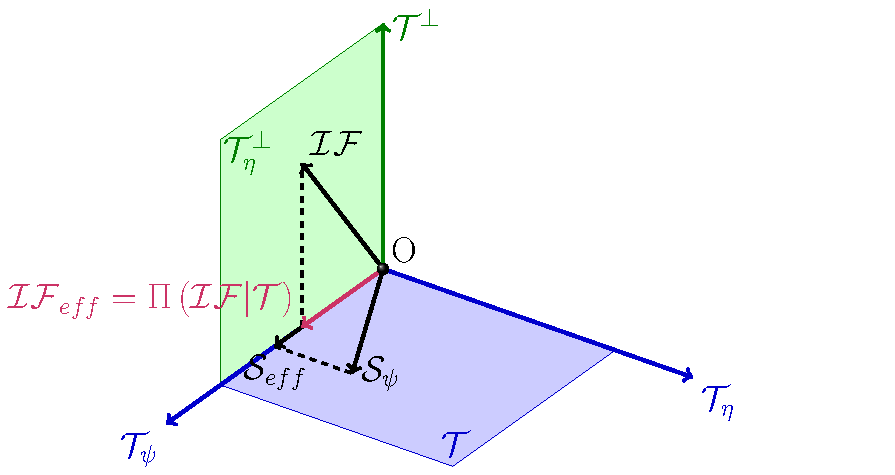
\includegraphics[width=0.8\textwidth]{./Figures/geometry.pdf}
\caption{\label{fig:geometry}Geometrical view of the influence function (\(\IF\)), the score (\(\Score\)), the efficient influence function (\(\IF_{eff}\)), the efficient score (\(\Score_{eff}\)) with respect to the tangent space for the parameter of interest \(\Tspace_{\psi}\) and the tangent space for the nuisance parameters \(\Tspace_{\eta}\).}
\end{figure}


So we just need to remove the composant of the naive influence
function that lies in the orthogonal of the tangent space:
\begin{align*}
\IF^{eff}_{\hat{\psi}} &= IF_{\hat{\psi}} - \Pi(IF_{\hat{\psi}}|\Tspace^{\perp}) \\
&= IF_{\hat{\psi}} - \Pi(IF_{\hat{\psi}}|\Tspace_2) 
\end{align*}



where \(\Pi(.|x)\) denotes the projection of \(.\) onto \(x\). We
first note that any element \(h\) of
the Hilbert space can be decomposed as:
\begin{align*}
h(Y,A,Z) &= h_1(Y,A,Z) + h_2(Y,A,Z) + h_3(Y,A,Z) \\
h_1 &= \Esp[h(Y,A,Z)|Z] \\
h_2 &= \Esp[h(Y,A,Z)|Z] - \Esp[h(Y,A,Z)|A,Z] \\
h_3 &= \Esp[h(Y,A,Z)|A,Z] - h(Y,A,Z)
\end{align*}
Theorem 4.5 in \cite{tsiatis2007semiparametric} shows that for any \(j
\in \{1,2,3\}\), \(h_j=\Pi(h|\Tspace_j)\). So:
\begin{align*}
\Pi(IF_{\hat{\psi}}|\Tspace_2) =& \Esp[IF_{\hat{\psi}}|Z] - \Esp[IF_{\hat{\psi}}|A,Z] \\
=& \Esp\left[\Esp\left[\frac{A}{\pi} \left(Y - \mu_1\right) - \frac{(1-A)}{1-\pi}\left(Y - \mu_0\right) \Big| A,Z\right] \Big| Z\right] \\
&- \Esp[\frac{A}{\pi} \left(Y - \mu_1\right) - \frac{(1-A)}{1-\pi}\left(Y - \mu_0\right) \Big| A,Z] \\
=& \frac{\Esp[A]}{\pi} \left(\Esp[Y|A=1,Z] - \mu_1\right) - \frac{\Esp[1-A]}{1-\pi}\left(\Esp[Y|A=0,Z] - \mu_0\right) \\
&- \left( \frac{A}{\pi} \left(\Esp[Y=1|A,Z] - \mu_1\right) - \frac{(1-A)}{1-\pi}\left(\Esp[Y|A=0,Z] - \mu_0\right)\right)  \\
=& \frac{\pi-A}{\pi} \left(\Esp[Y|A=1,Z] - \mu_1\right) - \frac{(1-\pi) - (1-A)}{1-\pi}\left(\Esp[Y|A=0,Z] - \mu_0\right) 
\end{align*}
which lead to the following expression for the efficient influence function:
\begin{align*}
\IF^{eff}_{\hat{\psi}} =& \frac{A}{\pi} \left(Y - \mu_1\right) + \frac{\pi-A}{\pi} \left(\Esp[Y|A=1,Z] - \mu_1\right) \\
&- \frac{(1-A)}{1-\pi}\left(Y - \mu_0\right) - \frac{(1-\pi) - (1-A)}{1-\pi}\left(\Esp[Y|A=0,Z] - \mu_0\right)  \\
=& \IF^{eff}_{\hat{\mu}_1} - \IF^{eff}_{\hat{\mu}_0}
\end{align*}
Solving \(\sum_{i=1}^n \IF^{eff}_{\hat{\mu}_1} = 0\) in \(\mu_1\) gives:
\begin{align*}
\sum_{i=1}^n\frac{A_i + \pi - A_i }{\pi}\tilde{\mu}_1 &= \sum_{i=1}^n \left( \frac{A_i Y_i}{\pi} + \frac{\pi-A_i}{\pi} \Esp[Y|A=1,Z] \right)\\
\tilde{\mu}_1 &= \frac{1}{n_1}\sum_{i=1}^n \left( A_i Y_i + (\pi-A_i) \Esp[Y|A=1,Z] \right) \\
              &= \hat{\mu}_1 + \frac{1}{n_1}\sum_{i=1}^n (\pi-A_i) \Esp[Y|A=1,Z]
\end{align*}
Similarly:
\begin{align*}
\tilde{\mu}_0 &= \frac{1}{n_0}\sum_{i=1}^n \left( (1-A_i) Y_i + ((1-\pi)-(1-A_i)) \Esp[Y|A=0,Z] \right) \\
              &= \hat{\mu}_0 + \frac{1}{n_0}\sum_{i=1}^n ((1-\pi)-(1-A_i)) \Esp[Y|A=0,Z]
\end{align*}
and:
\begin{align*}
\tilde{\psi} &= \tilde{\mu}_1 - \tilde{\mu}_0 \\
              &= \hat{\psi} + \frac{1}{n_1}\sum_{i=1}^n (\pi-A_i) \Esp[Y|A=1,Z] - \frac{1}{n_0}\sum_{i=1}^n ((1-\pi)-(1-A_i)) \Esp[Y|A=0,Z]
\end{align*}

\section{Relationship to the G-formula computation}
\label{sec:orga2231ff}

When performing a logistic regression including an intercept, A, and Z
the score equation is:
\begin{align*}
\sum_{i=1}^n X_i \left(Y_i - \frac{1}{1+exp(-X_i \theta)}\right) = 0
\end{align*}
where \(X_i = (1,A_i,Z_i)\) is the design matrix and
\(\theta=(\theta_1,\theta_A,\theta_Z)\) the set of model
parameters. We can in fact reparametrize it as \(X_i =
(1-A_i,A_i,Z_i)\) with
\(\theta=(\theta_{1-A},\theta_A,\theta_Z)\). Then the logistic
regression solves the following equations:
\begin{align*}
&\sum_{i=1}^n A_i \left(Y_i - \frac{1}{1+exp(-X_i \theta)}\right) = 0 \\
&\sum_{i=1}^n (1-n A_i) \left(Y_i - \frac{1}{1+exp(-X_i \theta)}\right) = 0
\end{align*}
i.e.
\begin{align*}
&\frac{1}{n} \sum_{i=1}^n \frac{A_i}{\pi} \left(Y_i - \frac{1}{1+exp(-\theta_{A}-Z_i \theta_Z)}\right) = 0 \\
&\frac{1}{n}  \sum_{i=1}^n \frac{1 - A_i}{1-\pi} \left(Y_i - \frac{1}{1+exp(-\theta_{1-A}-Z_i \theta_Z)}\right) = 0
\end{align*}
So the G-formula estimator is asymptotically equivalent to the efficient estimator:
\begin{align*}
\bar{\mu}_1 &= \frac{1}{n} \sum_{i=1}^n \frac{1}{1+exp(-\theta_{A}-Z_i \theta_Z)} \\
            &= \frac{1}{n} \sum_{i=1}^n \Esp[Y|A_i=1,Z_i] + o_p(1) \\
            &= \frac{1}{n} \sum_{i=1}^n \Esp[Y|A_i=1,Z_i] + \frac{A_i}{\pi}\left(Y_i - \Esp[Y|A_i=1,Z_i]\right) + o_p(1) \\
            &= \tilde{\mu}_1 + o_p(1)
\end{align*}
Because
\begin{align*}
\Esp[\frac{A}{\pi}\left(Y - \Esp[Y|A=1,Z]\right)] &= \Esp[\frac{A}{\pi}\left(Y - \Esp[Y|A,Z]\right)] \\
&= \Esp\left[\Esp\left[\frac{A}{\pi}\left(Y - \Esp[Y|A,Z]\right)\Big|A,Z\right]\right] \\
&= \Esp\left[\frac{\Esp[A]}{\pi}\left(\Esp[Y|A,Z] - \Esp[Y|A,Z]\right)\right] = 0
\end{align*}

\section{References}
\label{sec:org22dbe02}
\begingroup
\renewcommand{\section}[2]{}
\bibliographystyle{apalike}
\bibliography{bibliography}

\endgroup
\end{document}